\section{Skalarproduktet}\label{sec:scalar}
Ligesom med addition er dette også gennemgået på Mat A adgangskurset.
Multiplikation af en vektor, med en skalar $\alpha$, svarer til at gange på hver værdi i vektoren.
Dette kan eksemplificeres med vektoren $[3,4,7]$.
Hvis denne ganges med skalaren 5, gøres dette på følgende vis:
\begin{equation}
	\label{eqn:scalar}
	5[3,4,7] = [5\cdot3,5\cdot4,5\cdot7] = [15,20,35]
\end{equation}
Hvis der samtidig adderes en vektor på, følger dette de arritmetiske regler. 
Der ganges først, så adderes der.
Hvis en vektor ganges med et negativt tal, ændres fortegnet for alle elementer i vektoren.
Dette betyder at vektoren vil ændre orientering.
Samtidig gælder følgende for multiplikation af vektorer med ekstra skalarer:
\begin{equation}
	\label{eqn:scalar_mult}
	\alpha(\beta v)=(\alpha\beta)v
\end{equation}

\subsection{Linjer gennem origo}\label{ssec:lto}
Med vektorer kan linjer også tegnes fra origo.
Dette kan blandt andet gøres med følgende sæt af punkter.
\begin{equation}
	\label{eqn:origo}
	\set*{\alpha v; \alpha\in\mathrm{R},0\leq\alpha\leq1}
\end{equation}
Ovenstående sæt tenger en linje af punkter fra origo til $v$.
Med python koden vist i \cref{lst:python_plot} gives følgende plot
\begin{figure}[h]
	\centering
	
\includegraphics[width=0.5\textwidth]{img/vecplot.png}
	\caption{Plot fra udsnittet \cref{lst:python_plot}}
	\label{fig:plot_line}
\end{figure}
\lstinputlisting[
	language=Python,
	firstline=4,
	lastline=7,
	firstnumber=4,
	label=lst:python_plot,
	caption={Python kode til at generere plot i \cref{fig:plot_line}.\\Koden kan findes i ./labs/vectors/python\_plot.py}
]{labs/vectors/python_plot.py}

I kombination med at segmenter af linjer, kan samles til hele linjer og at der kan dannes uendelig mange skalar vektorer, kan vi danne figurer, når $\alpha$ strækker sig over flere tal.
Skalarprodukter $<1$ giver anledning til kopier af $v$, samtidig med at negative Skalarprodukter giver anledning til vektorer der peger i den anden retning.
Sættet af punkter $\set*{\alpha v;\alpha\in \mathrm{R}}$ strækker sig fra $-\infty;\infty$, og producerer derfor følgende plot:
\begin{figure}[h]
	\centering
	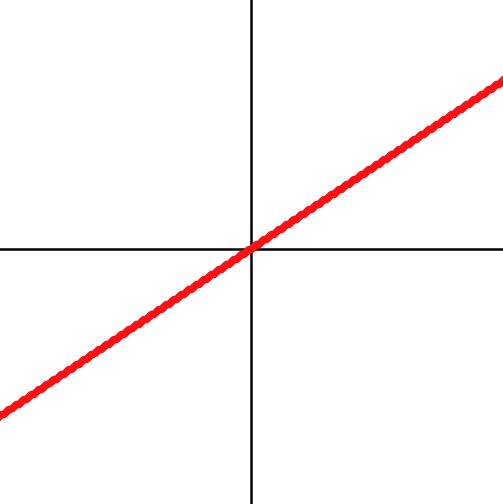
\includegraphics[width=0.5\textwidth]{img/thrh_origin.png}
	\caption{Sættet $\set*{\alpha v;\alpha\in \mathrm{R}}$ plottet i en graf.
	Både $x$ og $y$ aksen går fra $-\infty;\infty$}
	\label{fig:plot_through}
\end{figure}

Grafen i \cref{fig:plot_through} kan laves med følgende stykke python kode:
\lstinputlisting[
	language=Python,
	firstline=4,
	lastline=7,
	firstnumber=4,
	label=lst:scalar_plot,
	caption={Python kode til at generere plot i \cref{fig:plot_through}.\\Koden kan findes i ./labs/vectors/scalar\_plot.py}
]{labs/vectors/scalar_plot.py}
